%classe do documento Springer
\documentclass{llncs}

%%% user packages gerais %%%

\usepackage{amssymb}
\setcounter{tocdepth}{3}
\usepackage{graphicx}

\usepackage{url}
\urldef{\mailsa}\path|{drcinalli}@gmail.com|    
\urldef{\mailsb}\path|{lmarti}@ele.puc-rio.br|  
%\urldef{\mailsc}\path|{}@springer.com|    
\newcommand{\keywords}[1]{\par\addvspace\baselineskip
\noindent\keywordname\enspace\ignorespaces#1}

%cores
\usepackage{xcolor}
%letras gregas  grandes
\usepackage{upgreek}
%bib
\usepackage{natbib}
%margem
\usepackage{etoolbox}
\makeatletter
\patchcmd{\@addmarginpar}{\ifodd\c@page}{\ifodd\c@page\@tempcnta\m@ne}{}{}
\makeatother
\reversemarginpar
%blind text
\usepackage[english]{babel}
%\usepackage{blindtext}
\usepackage{lipsum}
%tabular
\usepackage{array}

%numero de pagina
%\pagestyle{headings}
%\setcounter{page}{1}
%\pagenumbering{roman}

%\usepackage{fancyhdr} 
%\fancyhf{}
%\cfoot{\thepage}
%\pagestyle{fancy}  
%\usepackage{fancyhdr}
%\fancyhf{}% clears headers and footers
%\fancyhead[EL]{Upper left corner}% Header on even pages (E), left (L)
%\fancyhead[OR]{Upper right corner}% Header on odd pages (O), right (R)
%\fancyhead[C]{Center}% Header on both pages, center (C)
%\renewcommand{\headrulewidth}{0pt}% Sets header rule to 0.4pt
%\fancyfoot[EL]{Lower left corner}% Footer on even pages (E), left (L)
%\fancyfoot[OR]{Lower right corner}% Footer on odd pages (O), right (R)
%\fancyfoot[C]{Center}% Footer on both pages, center (C)
%\renewcommand{\footrulewidth}{0pt}% Sets footer rule to 0pt
%\pagestyle{fancy}% Activates fancy page style
\usepackage{fancyhdr}
\pagestyle{fancy}
\fancyhf{} % clear all header and footer fields
\cfoot{\thepage}% ==>Tell LaTeX to make the center bottom empty
%\rfoot{\thepage}% ==>Tell LaTeX to put the page number at the right bottom
\renewcommand{\headrulewidth}{0pt}% ==> Set the line at the top of the page to 0pt.
%\fancyhead{}

% pseudocode
\usepackage{algorithm}
\usepackage{algpseudocode}


% math
\usepackage{amsmath}
\usepackage{multiobjective} 
\usepackage{appendix}

%figure
%\usepackage{float}
%\floatstyle{boxed}
%\restylefloat{figure}
% tables
\usepackage{hhline}
\usepackage{booktabs,mathptmx,siunitx}
\sisetup{input-symbols = {()},  % do not treat "(" and ")" in any special way
         group-digits  = false} % no grouping of digits
\newcommand{\ra}[1]{\renewcommand{\arraystretch}{#1}}
\usepackage{multirow,array}
\usepackage[section]{placeins}
\ExplSyntaxOn
\NewDocumentCommand{\longdash}{ O{2} }
 {
  --\prg_replicate:nn { #1 - 1 } { \negthinspace -- }
 }
\ExplSyntaxOff

\let\oldhat\hat
\renewcommand{\vec}[1]{\mathbf{#1}}
\renewcommand{\hat}[1]{\oldhat{\mathbf{#1}}}


% comeco do doc
\begin{document}


\mainmatter  % start of an individual contribution

% first the title is needed
\title{Miscellaneous}

% a short form should be given in case it is too long for the running head
\titlerunning{Miscellaneous}

% the name(s) of the author(s) follow(s) next
%
\author{Daniel Lopes Cinalli%
%\thanks{Please note that the LNBIP Editorial assumes that all authors have %used
%the western naming convention, with given names preceding surnames. This %determines
%the structure of the names in the running heads and the author index.}%
%\and Luis Mart\'{i}\and Nayat Sanchez-Pi
%\and Ana Cristina Bicharra Garcia
}
%
\authorrunning{Miscellaneous}
% (feature abused for this document to repeat the title also on left hand pages)

% the affiliations are given next
\institute{Universidade Federal Fluminense, Niter\'{o}i, Brazil\\
%\mailsa\\
%\mailsb\\
}
%\mailsc\\
%\url{http://www.springer.com/lncs}}

%
% NB: a more complex sample for affiliations and the mapping to the
% corresponding authors can be found in the file "lnbip.dem",
% that is contained in the LNBIP LaTeX support package.
%

%\toctitle{Lecture Notes in Business Information Processing}
%\tocauthor{Authors' Instructions}
\maketitle

\tableofcontents

\newpage
\section{Mathematical Model}

\subsection{Bi-objective}\label{sec:biobjective}
The problem is formally represented as: 



%f1
\begin{equation}
\min \sum\limits_{i=1}^{N} \sum\limits_{j=1}^{M} \sigma_{ij}d_{ij} + \sum\limits_{j=1}^{M}c_j\mu
\end{equation}


%f2
\begin{equation}
\max \sum\limits_{i=1}^{N} \sum\limits_{j=1}^{M} \sigma_{ij}v_j
\text{  (or)  }
\max \sum\limits_{i=1}^{N} \sum\limits_{j=1}^{M} \sigma_{ij}h(v_j, a_i)
\end{equation}

%%Poderia me ajudar nesse parágrafo? acho q não está bom %%
Let $\mu$ be the cost of one processing  unit, $v$ the productive capacity of one processing unit linked to one resource area, $a$ the  available resource for the area, $h$ a function to outcome the minimum of two values, $M$ a set of available positions to processing units, $N$ a set of available positions to resource areas and $D$ a distance matrix $(d_{ef})_{n_{x}m}$, where $n \in N$ and $m \in M$. The decision variables are the processing unit $c_j$ ($j \in M$) that assumes $1$ if it is placed at position $j$ or $0$ otherwise and $\sigma_{ij}$ that assumes $1$ if there is a link between the resource area $g$ at position $i \in N$ and the processing unit at position $j \in M$. 



%production unit
\begin{equation}
 c_j = \left\{
  \begin{array}{l l}
    1 & \quad \text{if the processing unit is placed}\\
    0 & \quad \text{otherwise}
  \end{array} \right.
\end{equation}

%link unit vs. gateway
\begin{equation}
 \sigma_{ij} = \left\{
  \begin{array}{l l}
    1 & \quad \text{if there is a link between }g_i \text{ and }c_j\\
    0 & \quad \text{otherwise}
  \end{array} \right.
\end{equation}

\subsection{Tri-objective}

The problem is formally represented bellow: 


%f1
\begin{equation}
\min \sum\limits_{i=1}^{N} \sum\limits_{j=1}^{M} \sigma_{ij}d_{ij} 
\end{equation}


%f2
\begin{equation}
\min \sum\limits_{j=1}^{M}c_j\mu
\end{equation}


%f3
\begin{equation}
\max \sum\limits_{i=1}^{N} \sum\limits_{j=1}^{M} \sigma_{ij}v_j
\text{  (or)  }
\max \sum\limits_{i=1}^{N} \sum\limits_{j=1}^{M} \sigma_{ij} h(v_j, a_i)
\end{equation}


\subsection{Constraints}

Let $P$ the available positions to one specific area, $q$ the maximum number of  resource areas allowed, $k$ the maximum number of  processing  unit allowed and $r$ the minimum distance between the processing unit and the resource area. The constraints are defined as:   

%restricao de quantidade da unidade de producao menor que a area de producao
\begin{equation}
 1 \leq k \leq  q
\end{equation}


%restricao de atendimento da unidade de producao
\begin{equation}
 1 \leq \sum\limits_{j=1}^{M} c_j \leq k
\end{equation}



%%restricao de atendimento do gateway na area
%\begin{equation}
%\sum\limits_{i=1}^{P} g_i = 1
%\end{equation}
  
%restricao de atendimento de que o gateway tenha exatamente 1 destino
\begin{equation}
\sum\limits_{i=1}^{P} \sigma_{ij}=1, j=1,\ldots,M
\end{equation}


%restrição de distancia mínima
\begin{equation}
 \sum\limits_{i=1}^{N} \sum\limits_{j=1}^{M} \sigma_{ij}\geq r
\end{equation}

Considering the link $\sigma_{ij}$ between one resource area $g_i$ and the processing unit $c_j$, a geometric interpretation of  $\sigma_{ij}$ transforms the link into a $2$-dimensional space line segment $\overline{g_ic_j}$ defined by two distinct points $\left(x_1,y_1\right)$ for $g_i$  and $\left(x_2,y_2\right)$ for $c_j$. Another constraint to the problem states that the links (lines segments) in the solution cannot intercept each others. Therefore, given two links and their respective points: $\left(x_1,y_1\right)$ and $\left(x_2,y_2\right)$ for $\overline{g_ic_i}^A$; $\left(x_3,y_3\right)$ and $\left(x_4,y_4\right)$ for $\overline{g_ic_i}^B$; the intersection $P$ of two lines segments is verified if each of the two pairs of cross products below have different signs (or one cross product in the pair is 0).  The Sweeping algorithm \cite{Berg:2008:CGA:1370949} deals with a set of $n$ line segments in the plane and avoids testing pairs of segments that are far apart.


\begin{equation}
\left(p_1-p_4\right)\times\left(p_3-p_4\right) \And \left(p_2-p_4\right) \times \left(p_3-p_4\right)
\end{equation}

\begin{equation}
\left(p_3-p_2\right)\times\left(p_1-p_2\right) \And \left(p_4-p_2\right) \times \left(p_1-p_2\right)
\end{equation}

%their bounding box do not intersect: $\left(x_4<x_1\right) \vee \left(x_3>x_2\right) \vee \left(y4<y_1\right) \vee \left(y_3>y_2\right)$; or the two pairs of cross products have different signs (or one cross product in the pair is 0).



 
%restrição para não cruzar
%\begin{equation}
%\textcolor{red}{
%\sum\limits_{i=1}^{N} \sum\limits_{j=1}^{M}
%\texttt{ links can't cross each other!}
%}
%\end{equation}


%In the end, the sweep alg (ref) will do the job

\subsection{Data Structure}


In genetic algorithms, the individual structure is referred to as genotype, gene or chromosome and the values that a chromosome may take on are named as alleles. The computational representation for the problem in section \ref{sec:biobjective} considers the processing unit as a tuple $c_i=<x, y, t>$; where $c_i \in C=\left\{c_1,...,c_k\right\}$, $t$ is the type of the unit, $x \text{ and }y$ are the Cartesian coordinates of the position. The resource area is represented by the tuple $a_i=<x, y, l>$; where $a_i \in A=\left\{a_1,...,a_q\right\}$, $l$ is a index that links the resource area $a_i$ to the unit $c_i$. Thus, the chromosome encoding is the aggregation of these tuples regulated by $q$ resource areas and $k$ processing units.



\begin{figure}
\centering
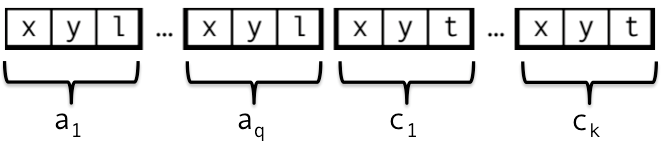
\includegraphics[height=.5in,width=3in]{gene1.png}
\caption{Chromosome encoding for the problem.}
\label{fig:gene}
\end{figure}
\FloatBarrier


%\textcolor{blue}{Individual representation ... ....}


\section{Foundations}

\marginpar{\textcolor{blue}{Evolutionary Alg.}}
Evolutionary algorithms (EA) are inspired in Darwinian principles of natural evolving systems to automated problem solving \cite{back-1996:evolutionary-algorithms}. The methods are population-based and cover a wide range of problems that includes constraint satisfaction and combinatorial optimization. Its typical components are a space of individuals $I$ to be considered as candidate solutions, a problem-specific fitness function of individuals $F: I \rightarrow \mathbb{R}$ and some mechanisms  for search strategy. The underlying idea behind EAs can be viewed as a crossover-mutation-fitness evaluation-selection loop until a termination criterion is reached, such as: a candidate with acceptable quality or a previous computational constraint. High-level  framework uses $\mu$ and $\lambda$ to represent  parent and offspring population sizes. Therefore, a population $P$ of individuals $a \in I$ at generation $t$, $P(t)=\left(a_1(t),\ldots, a_\mu(t)\right) \in I^\mu$, applies selection, mutation, and crossover operators respectively described as: $s: I^\lambda \rightarrow I^\mu$, $m: I^k \rightarrow I^\lambda$ and $r: I^\mu \rightarrow I^k$.  





\marginpar{\textcolor{blue}{Hypervolume}}
The quality of MOEAs' trade-off fronts can be quantitatively evaluated by many different techniques. The hypervolume or $S$-metric \cite{emmerich2005emo, zitzler1999multiobjective} is a quantitative measure of the space covered by the non-dominated points.   It represents the union of hypercubes $a_i$ defined by a non-dominated point $m_i$ and a reference point $x_{ref}$ as defined in (\ref{eqn:hyp}).  

\begin{equation}\label{eqn:hyp}
\begin{array}{rl}
 S(M) & = \Lambda(\{\bigcup_{i} a_i|m_i \in M\}) \\
      & = \Lambda( \bigcup_{m \in M} \{x|m \dom x \dom x_{ref}\}).\\
\end{array}
\end{equation}

A second measure widely used is the coverage of two sets \cite{zitzler1999multiobjective};
\begin{equation}
 C(X', X'')=\frac{|\{a' \in X'';\exists a' \in X': a' \dom a''\}|}{|X''|},
\end{equation}
where $X'$, $X'' \subseteq X$ are two sets of decision vectors and function $C$ maps the percentage of domination from one set to another in the interval $[0,1]$. Although convex regions may be preferred by the hypervolume, it can be used independently to evaluate the performance of different multi-objective algorithms. The coverage of two sets technique has no restriction related to the shape of Pareto front, but it does not express how much better one set is over the other.


\marginpar{\textcolor{blue}{Mixture Model}}
A mixture model is a probabilistic model to reveal distributions of observations in the overall population \cite{Padhraic,barber2012bayesian}. Given a data set $D=\{\vec{x}_1,\ldots,\vec{x}_N\}$ where $\vec{x}_i$ is a $d$-dimensional vector measurement with the points created from density $p(\vec{x})$, a finite mixture model is defined as:

\begin{equation}\label{eqn:mix1}
 p\left( \vec{x}|\Theta\right)=\sum\limits_{k=1}^{K}\alpha_kp_k\left(  \vec{x}|z_k,\theta_k \right) 
\end{equation} 

Let $K\geq1$ be the number of components, $p_k\left(  \vec{x}|z_k,\theta_k \right)$ be the mixture components where each $k$ is a density or distribution over $p\left(\vec{x}\right)$ and parameters $\theta_k$, $\vec{z}=\{z_1,\ldots,z_k\}$ be a $K$-ary random variable defining the identity of the mixture component that produced $\vec{x}$ and $\alpha_k=p_k\left(  z_k \right)$ are the mixture weights representing the probability that $\vec{x}$ was generated by component $k$. Hence, the parameters for a mixture model is $\Theta = \{ \alpha_1,\ldots,\alpha_K,\theta_1,\ldots,\theta_K\}$, $1\leq k \leq K$.

In a Gaussian mixture model, each of the $K$ components is a Gaussian density with parameters $\theta=\{\vec{\mu}_k,\Sigma_k\}$, $\vec{x} \in \mathbb{R}^d$ and function as:

\begin{equation}\label{eqn:gaussian1}
p_k\left( \vec{x}|\theta_k\right) = \frac{1}{ \left(2\pi\right)^{d/2} |\Sigma_k|^{1/2}}e^{-\frac{1}{2}\left( \vec{x} - \vec{\mu}_k\right)^t \Sigma^{-1}_k\left(\vec{x}-\vec{\mu}_k\right)}
\end{equation} 


\marginpar{\textcolor{blue}{Expec. Maximization}}
The expectation maximization (EM) algorithm \cite{dempster1977maximum} for Gaussian mixture is a particular way of implementing the maximum likelihood estimation in probabilistic models with incomplete or missing data values. EM learns the parameters $\theta_k$ guessing a distribution for the unobserved data and finds the cluster to which a singular chromosome  most likely belongs. It starts with an initial estimation of $\Theta$ and iterates between E-step and M-step of the algorithm to update $\Theta$ until convergence. 

E-step estimates the posterior distribution of the latent variables taking into account  the current parameters and the observed data. The membership weight $w_{ik}$ computes the probability of all data points $\vec{x}_i$ to the mixture components $k$. In the M-Step, the algorithm uses the calculated membership weights to find new model parameters values.


\begin{equation}\label{eqn:membership}
w_{ik} = p\left(z_{ik}=1|\vec{x}, \Theta\right) = \frac{p_k\left(  \vec{x}|z_k,\theta_k \right)\alpha_k}{\sum_{m=1}^{K}p_m\left(  \vec{x}|z_m,\theta_m \right)\alpha_m},  1\leq k \leq K,  1\leq i \leq N
\end{equation} 


After E and M steps the  convergence is computed using the value of the log-likelihood $\text{log } l\left(\Theta\right)$. The algorithm stops when there are no significant changes in the convergence from one iteration to the next.


\begin{equation}\label{eqn:loglike}
\text{log } l\left(\Theta\right) = \sum\limits_{i=1}^{N} \text{log } p\left(  \vec{x}|\theta \right)= \sum\limits_{i=1}^{N} \left(\text{log }\sum\limits_{k=1}^{K} \alpha_kp_k\left(  \vec{x}|z_k,\theta_k \right) \right)
\end{equation} 



 
 
 
%Multivariate Gaussian mixture model: A Bayesian Gaussian mixture model is commonly extended to fit a vector of unknown parameters (denoted in bold), or multivariate normal distributions. In a multivariate distribution (i.e. one modelling a vector x with N random variables) one may model a vector of parameters (such as several observations of a signal or patches within an image) using a Gaussian mixture model prior distribution on the vector of estimates given by (fonte: mixture model no Wiki)


\section{Results of EMOA (without COIN integration)}

Using the 20x20 and 50x50 scenarios, tables \ref{tab:20x20avg} and \ref{tab:20x20comp} show the best results after 40 independent executions per EA. Every MOEA's execution performed 400 generations for 200 individuals (population) in the 20x20 domain and 900 generations for 700 individuals in 50x50. Each EA's execution returns a Pareto front $F$ based on the union of all previous non-dominant sets throughout the generations: $F_i=nd\left(Pi  \cup  F_{i-1}\right)$; where $P_i$ is the set of points for generation $i$, $F_{i-1}$ is the Pareto front from the previous one and $nd$ is a dominance function. Considering all Pareto fronts produced ($m=40$, in this experiment) and $h$ the hypervolume function, $\bar{H}= \frac{\sum\limits_{i=1}^{m}h(F^i)}{m}$ is the average hypervolume used to analyse the best operators and algorithm for the problem.

The crossover rate is 0.30 and the mutation rate is 0.10.  Due to the problem's constraints, after those operations some new individuals might have invalid combinations of units and gates positions. Four strategies were implemented to repair the offspring (see section \ref{sec:fix}): \textit{fix random} - which randomly repairs gates' position, units' position and links; \textit{fix greedy} - which repairs units' position by the closest distance to the area; \textit{no fix loop} - does not repair, but rejects the invalid individual and keeps selecting new individuals until population is complete; \textit{no fix} - does not repair any individual, just assigns a bad fitness value to it.  

%Discarded crossover techniques: \textit{Partialy Matched} - index vector, it does not fit to my structure; \textit{Uniform Partialy Matched} - index vector, it does not fit to my structure; \textit{Ordered} - index vector, it does not fit to my structure; \textit{Blend} - expects floating points; \textit{Simulated Binary} - expects floating points; \textit{Simulated Binary Bounded} - expects floating points; \textit{Messy One Point} - change the individuals size.

%Discarded mutation techniques: \textit{Gaussian} - not applicable to my dna; \textit{Shuffle Indexes }- vector of indexes; \textit{Polynomial Bounded} - floating points.


\begin{table*}
\caption{20x20 average hypervolume analysis for \textit{fix randon} strategy}
\label{tab:20x20avg}
\centering
\begin{tabular}{@{}lclclclc c @{}}
\toprule

• & \phantom{abc}  & Crossover & \phantom{abc}  & Mutation & \phantom{abc}  & Selection & \phantom{abc} & \multicolumn{1}{c}{Hypervolume}\\
 \midrule


\multirow{6}{*}{$\bar{H}$} & & Two-Point&  &  & & \multirow{3}{*}{NSGA-II} & &  0.5922 \\
 & & One-Point&  &  & &  & &  0.5795 \\
 & & Uniform&  &  & &  & &  0.5939\\\hhline{~~=======}
 & & \multirow{3}{*}{Uniform}&  & Flip Bit & & \multirow{3}{*}{NSGA-II} & &  0.5990 \\
 & & &  & Uniform Int & &  & &  \bf{0.6021} \\
 & & &  & Shuffle Indexes & &  & &  0.6005 \\


 \bottomrule
\end{tabular} 
\end{table*}



\begin{table*}
\caption{20x20 average hypervolume analysis for all strategies}
\label{tab:20x20comp}
\centering
\begin{tabular}{@{}lclclc l@{}}
\toprule

• & \phantom{abc}  & Fix & \phantom{abc}  & Selection & \phantom{abc} & \multicolumn{1}{c}{Hypervolume}\\
 \midrule


\multirow{8}{*}{$\bar{H}$} & & \multirow{2}{*}{Randon} & & NSGA-II & &  \bf{0.6021} \\
 & &  & & SPEA-2 & &  0.5874 \\[2ex]

 & & \multirow{2}{*}{Greedy}  & & NSGA-II & &  0.6025 \\
 & &  & & SPEA-2 & &   0.5932 \\[2ex]


 & & \multirow{2}{*}{No Fix Loop}  & & NSGA-II & &  0.5983 \\
 & &  & & SPEA-2 & &  0.5494 \\[2ex]


 & & No Fix &  & NSGA-II & &  0.5815 \\
 & &  & & SPEA-2 & &  0.5372 \\

 \bottomrule
\end{tabular} 
\end{table*}

\FloatBarrier

Figure  \ref{fig:box1} reports the distribution of results comparing different multi-objective genetic algorithms. For this problem, NSGA-II returned better outcomes than SPEA2 and the values are more concentrated to the mean. Figure  \ref{fig:map1} demonstrates two solutions from Pareto-optimal set composed of six resource areas (gray rectangles) and processing units (coloured circles). All resource areas are connected to only one unit in an optimal arrangement regarding the two objectives: cost and production. 


 
\begin{figure}
\centering
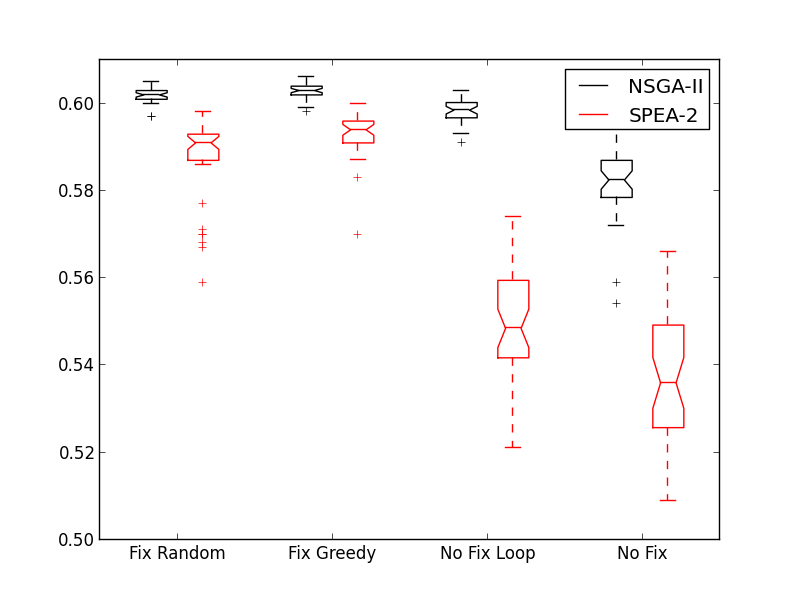
\includegraphics[height=3in,width=3in]{box2.png}
\caption{20x20 distribution of results after simulations}
\label{fig:box1}
\end{figure}
\FloatBarrier


\begin{figure}
\centering
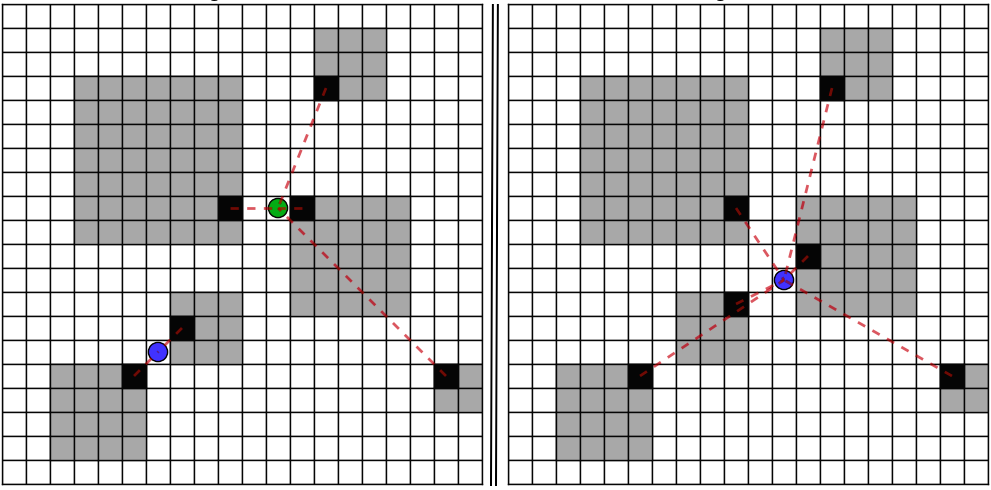
\includegraphics[height=3in,width=5in]{mapsolution1.png}
\caption{Evolutionary algorithm solution for six resource areas.}
\label{fig:map1}
\end{figure}
\FloatBarrier




%\subsection{500x500}
%\newpage
%\textbf{500x500}
%
%Testar!


\subsection{Pareto-optimum front}

The Pareto-optimal front for this real-world problem is calculated after 140 independent executions per EA. Considering all Pareto fronts $P^i$ achieved, $P^\ast$ is the set resulted after the dominance function $nd$ over all $P^i$, such that: $ P^{\ast}= nd(P^i), i=1,\ldots,m$ (in this case, $m=140$). The best non-dominated set $P^b$ from all executions is compared to $P^{\ast}$ in terms of convergence and diversity \cite{deb2002fast}. The experiment used the NSGA-II algorithm, uniform crossover and uniform integer mutation because this configuration achieved the best results in table \ref{tab:20x20avg}.


\begin{table*}
\caption{Comparation between 20x20 Pareto-optimum front  and the best MOEA's solution}
\centering
\begin{tabular}{@{}lclclclcl @{}}
\toprule

 & \phantom{abc}  & Hypervolume & \phantom{abc}  & \multicolumn{1}{m{1.7cm}}{Optimum Convergence} & \phantom{abc} & \multicolumn{1}{m{1.5cm}}{Optimum  Diversity}\\
 \midrule

 $P^{\ast}$ &  & 0.6080 &  & \multicolumn{1}{c}{\longdash[2]} & & \multicolumn{1}{c}{\longdash[2]} \\
 $P^{b}$ & & 0.6058 & & 0.7835 & & 1.0322  \\
 
 \bottomrule
\end{tabular} 
\end{table*}

\FloatBarrier


\begin{table*}
\caption{Comparation between 50x50 Pareto-optimum front  and the best MOEA's solution}
\centering
\begin{tabular}{@{}lclclclcl @{}}
\toprule

 & \phantom{abc}  & Hypervolume & \phantom{abc}    & \multicolumn{1}{m{1.7cm}}{Optimum Convergence} & \phantom{abc} & \multicolumn{1}{m{1.5cm}}{Optimum  Diversity}\\
 \midrule

 $P^{\ast}$ & & 0.7568 &  & \multicolumn{1}{c}{\longdash[2]}  & & \multicolumn{1}{c}{\longdash[2]}   \\
 $P^{b}$ & & 0.7565 &  & 0.0212 & & 1.5378  \\

 
 \bottomrule
\end{tabular} 
\end{table*}

\FloatBarrier


\section{Algorithm}\label{sec:algorithms}

ICIEA implements collective pairwise comparisons of scenarios into the optimization search for the resource placement problem explained in section \ref{sec:biobjective}. The approach iteratively suspends  the evolution to ask users for their preferred individuals in the population. Based on the group's subjectivity and cognition, all the population fitness values are recalculated and reinstated for next generations of MOEA. The algorithm is presented as follows:


\begin{algorithm}
\caption{ICIEA algorithm}
\label{alg:iciea}
\begin{algorithmic}[1]

\State $generation\gets num generation$\Comment{number of generations} 
\State $block\gets subset generation$\Comment{number of generations before pairwise}
\While{$generation$}

	\While{$block$}
		\State $offspring\gets \textbf{Tournament}(pop)$\Comment{based on dominance}
		\State $offspring\gets \textbf{Crossover}(offspring)$
		\State $offspring\gets \textbf{Mutation}(offspring)$
		\State $pop\gets \textbf{NSGA-II}(offspring)$
	\EndWhile
	\State $comparisons\gets \textbf{CollectivePairWise}(F^i) $\Comment{$F^i$ is the actual Pareto front}
	\State $\Theta\gets \textbf{ExpectatiomMaximization}(comparisons)$\Comment{$\Theta=\{\theta_{pro},\theta_{anti}\}$}
	\State $pop\gets \textbf{FitnessRecalculation}(pop,\Theta)$
\EndWhile

\end{algorithmic}
\end{algorithm}

\FloatBarrier

Considering the opposed objectives of cost and production (section \ref{sec:biobjective}), the collective pairwise comparisons represent sample observations that highlight points in the search space throughout the evolution.   In this case, however, there is an unobserved latent factor. The selected individuals may be most likely associated with a pro-cost or anti-cost (pro-production)  cluster, but, as the comparisons are anonymous, the previous tendencies and the distribution of the unobserved data are completely unknown. Hence, the EM algorithm finds a mixture of one-dimensional Gaussian distributions for $K=2$ components: $\theta_{pro}, \theta_{anti}$. The expression patterns for each cluster define the membership of the observations and use that probability to adjust a certain amount $\Psi$ to the fitness values. Algorithm \ref{alg:icieafitness} presents the fitness recalculation. 


\begin{algorithm}
\caption{ICIEA Fitness Recalculation}
\label{alg:icieafitness}
\begin{algorithmic}[1]
\Procedure{FitnessRecalculation}{$pop,\Theta$}
\State $\theta_{pro}\gets\Theta[0] $\Comment{$\theta=\{\mu,\sigma^2\}$}
\State $\theta_{anti}\gets\Theta[1] $
\ForAll{$individual$ \textbf{ in } $pop$}
	\State $cost \gets individual\_fitness[cost]$
	\State $p_{cost} \gets \textbf{GaussianDensity}(\theta_{pro},cost)$\Comment{membership to $\theta_{pro}$}
	\State $ \Psi= \mid p_{cost}.\sigma_{pro}^2.\textbf{zscore}(cost,\theta_{pro})\mid$
	\State $individual\_fitness[cost] += \Psi$
	\State

	\State $anticost \gets individual\_fitness[prod]$
	\State $p_{anticost} \gets \textbf{GaussianDensity}(\theta_{anti},anticost)$\Comment{membership to $\theta_{anti}$}
	\State $ \Psi= \mid p_{anti}.\sigma_{anti}^2.\textbf{zscore}(anticost,\theta_{anti})\mid $
	\State $individual\_fitness[prod] += \Psi$

\EndFor

\State \textbf{return} $pop$
\EndProcedure
\end{algorithmic}
\end{algorithm}

\FloatBarrier


Unlike $K$-means where data point must exclusively belong to one cluster center, Gaussian mixture model offers the possibility of many association for one unique point and this characteristic benefits the increase strategy of the fitness for distinct objectives.



%One possible model of such prices would be to assume that the prices are accurately described by a mixture model with K different components, each distributed as a normal distribution with unknown mean and variance, with each component specifying a particular combination of house type/neighborhood. Fitting this model to observed prices, e.g., using the expectation-maximization algorithm, would tend to cluster the prices according to house type/neighborhood 
 
% posso estimar os priors baseado na informação de perfil, não?
 

\newpage
\appendix
\section{Appendix: Fix Algorithms}\label{sec:fix}
Four strategies were implemented to repair the offspring after genetic operations. Their algorithms are present as follows: \textit{fix random} in algorithm \ref{alg:fixrandom} - which randomly repairs gates' position, units' position and links; \textit{fix greedy} in algorithm \ref{alg:fixgreedy} - which repairs units' position by the closest distance to the area; \textit{no fix loop} in algorithm \ref{alg:nofixloop} - does not repair, but rejects the invalid individual and keeps selecting new individuals until population is complete; \textit{no fix} in algorithm \ref{alg:nofix} - does not repair any individual, just assigns a bad fitness value to it.  


\begin{algorithm}
\caption{ICIEA fix random}
\label{alg:fixrandom}
\begin{algorithmic}[1]
\Procedure{FixRandom}{$invalids$}


\ForAll{$individual$ \textbf{ in } $invalids$}
	\State $units \gets \textbf{GetUnits}(individual)$\Comment{processing units  from chromosome} 			
	\State $areas \gets \textbf{GetAreas}(individual)$\Comment{resource areas from chromosome}
	\State
	\ForAll{ $position$ \textbf{ in }$units$}\Comment{fix processing units}
		\If {$wrong\_position$}
			\State $position \gets new\_position$\Comment{random}
		\EndIf 
	\EndFor
	\ForAll{ $position$ \textbf{ in }$areas$}\Comment{fix resource area}
		\If {$wrong\_position$}
			\State $position \gets new\_position$
		\EndIf 
	\EndFor
	\ForAll{ $area\_link$ \textbf{ in }$areas$}\Comment{fix links between area and unit}
		\If {$wrong\_area\_link$}
			\State $area\_link \gets \textbf{RandomUnitLink}()$
		\EndIf 
	\EndFor
\EndFor
\EndProcedure
\end{algorithmic}
\end{algorithm}

\FloatBarrier

\begin{algorithm}
\caption{ICIEA fix greedy}
\label{alg:fixgreedy}
\begin{algorithmic}[1]
\Procedure{FixGreedy}{$invalids$}


\ForAll{$individual$ \textbf{ in } $invalids$}
	\State $units \gets \textbf{GetUnits}(individual)$\Comment{processing units  from chromosome} 			
	\State $areas \gets \textbf{GetAreas}(individual)$\Comment{resource areas from chromosome}
	\State
	\ForAll{ $position$ \textbf{ in }$units$}\Comment{fix processing units}
		\If {$wrong\_position$}
			\State $position \gets new\_position$\Comment{random}
		\EndIf 
	\EndFor
	\ForAll{ $position$ \textbf{ in }$areas$}\Comment{fix resource area}
		\If {$wrong\_position$}
			\State $position \gets new\_position$
		\EndIf 
	\EndFor
	\ForAll{ $area\_link$ \textbf{ in }$areas$}\Comment{fix links between area and unit}
		\If {$wrong\_area\_link$}
			\State $area\_link \gets \textbf{ClosestUnitLink}()$
		\EndIf 
	\EndFor
\EndFor
\EndProcedure
\end{algorithmic}
\end{algorithm}

\FloatBarrier


\begin{algorithm}
\caption{ICIEA fix loop}
\label{alg:nofixloop}
\begin{algorithmic}[1]
\State $still\_invalids \gets len(pop)$
\While{$still\_invalids$}

	\State $offspring\gets \textbf{Tournament}(pop)$
	\State $offspring\gets \textbf{Crossover}(offspring)$
	\State $offspring\gets \textbf{Mutation}(offspring)$
	\State $still\_invalids \gets \textbf{Invalids}(offspring)$\Comment{number of invalids individuals}

\EndWhile
\State $pop\gets \textbf{NSGA-II}(offspring)$
\end{algorithmic}
\end{algorithm}

\FloatBarrier


\begin{algorithm}
\caption{ICIEA no fix}
\label{alg:nofix}
\begin{algorithmic}[1]
\Procedure{NoFix}{$invalids$}


\ForAll{$individual$ \textbf{ in } $invalids$}
	\State $individual\_fitness[cost] \gets  \infty$
	\State $individual\_fitness[prod] \gets  \infty$
\EndFor
\EndProcedure
\end{algorithmic}
\end{algorithm}

\FloatBarrier

\section{Appendix: ICIEA Gamification}

\begin{figure}
\centering
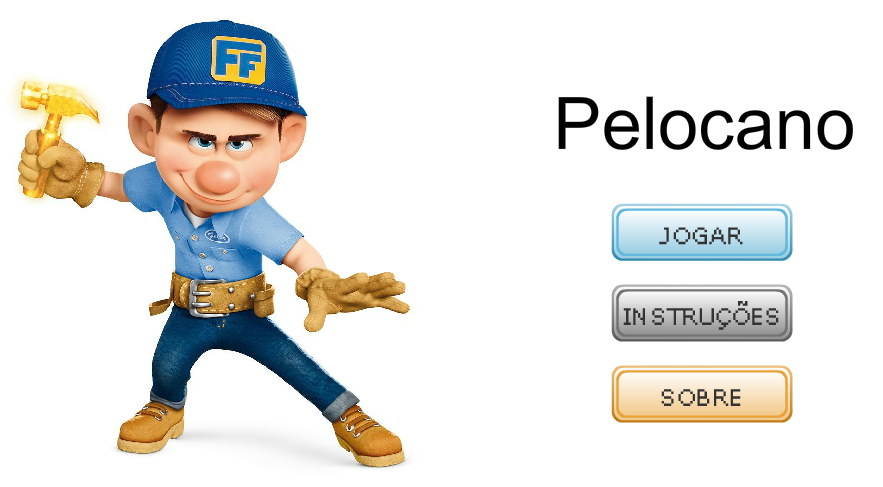
\includegraphics[height=2.5in,width=3in]{pelocano1.png}
\caption{Gamification first screen}
\label{fig:pelocano1}
\end{figure}
\FloatBarrier

\begin{figure}
\centering
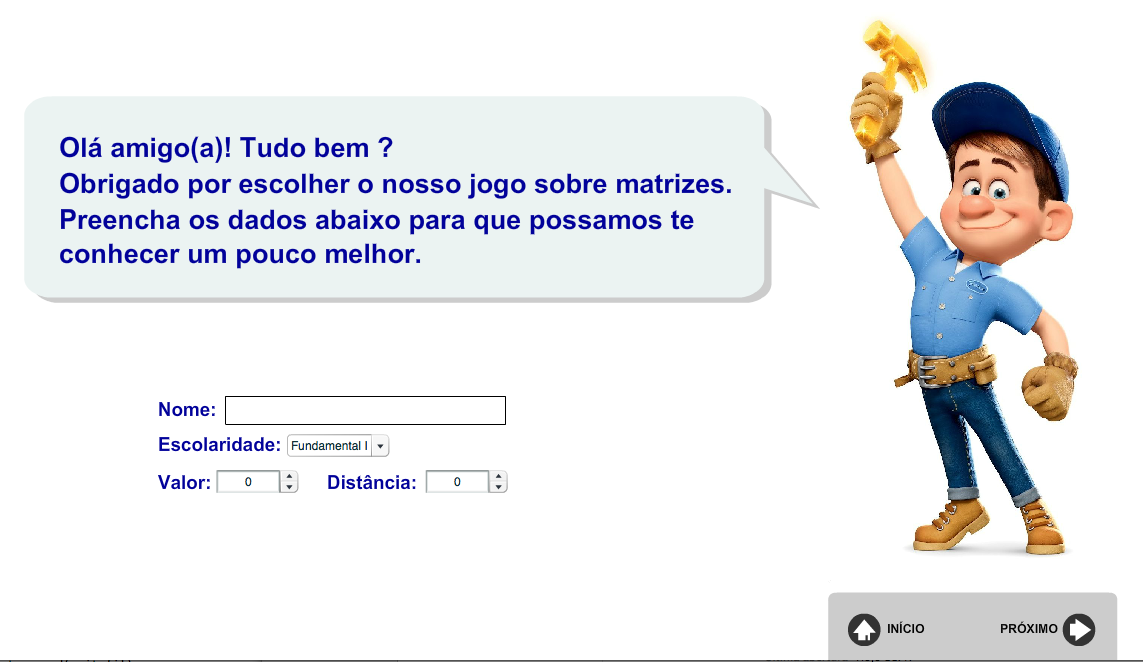
\includegraphics[height=2.5in,width=5in]{pelocano2.png}
\caption{User's profile }
\label{fig:pelocano1}
\end{figure}
\FloatBarrier

\begin{figure}
\centering

\includegraphics[height=2.5in,width=3in]{pelocano3.png}
\caption{User's profile }
\label{fig:pelocano3}
\end{figure}
\FloatBarrier

\begin{figure}
\centering
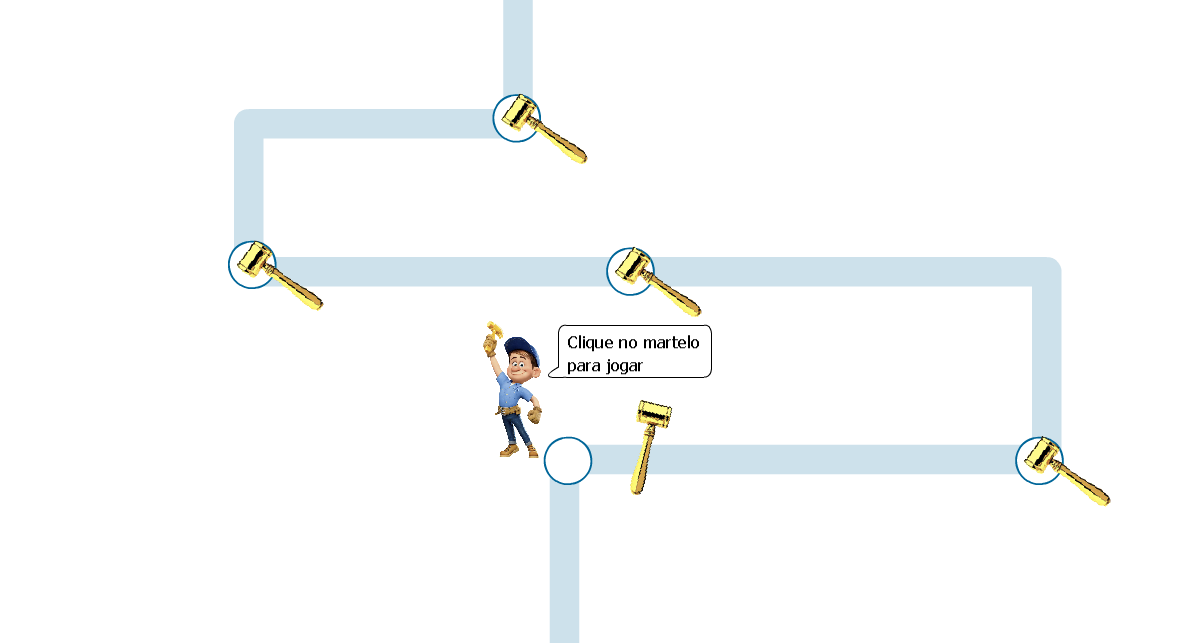
\includegraphics[height=1.6in,width=3in]{pelocano5.png}
\caption{Pairwise comparisons}
\label{fig:pelocano1}
\end{figure}
\FloatBarrier

\begin{figure}
\centering
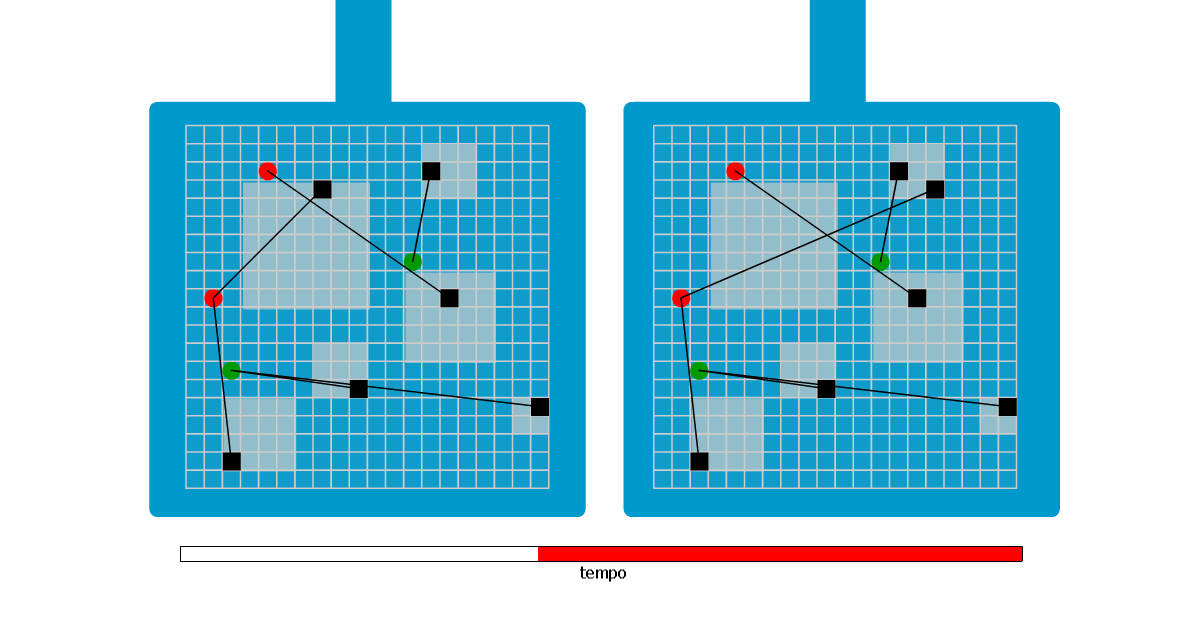
\includegraphics[height=1.6in,width=3in]{pelocano6.png}
\caption{Pairwise comparisons}
\label{fig:pelocano1}
\end{figure}
\FloatBarrier

\section{Appendix: ER model}

\begin{figure}
\centering
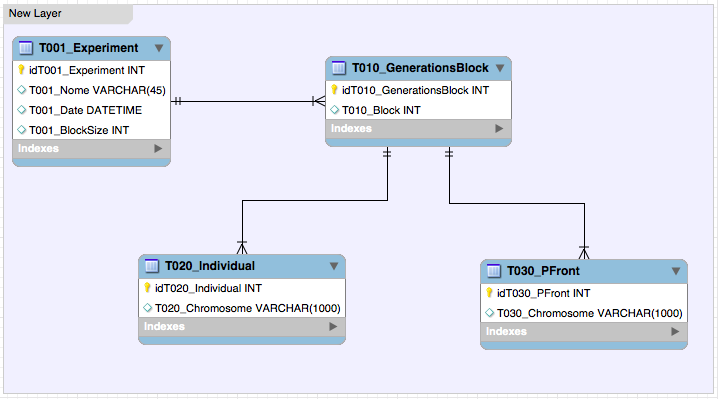
\includegraphics[height=2.9in,width=5in]{er.png}
\caption{ICIEA ER model}
\label{fig:er}
\end{figure}
\FloatBarrier

\section{Appendix: Multiattribute Utility}

Formally represented as utility functions $U_1(x_1),...,U_m(x_m)$ to $m$ different attributes $x_1$ to $x_m$. Each function takes 0 to the worst and 1 to the best level of an objective.

The utility function is:
 

%f1
\begin{equation}
U(x_1,...,x_m)=k_1U_1(x_1)+...+k_mU_m(x_m)=\sum\limits_{i=1}^{m} k_iU_i(x_i)
\end{equation}


subject to 

\begin{equation}
 \sum\limits_{i=1}^{m} k_i=1 
\end{equation}

where 


\begin{equation}
U_i(x) = \frac{x-worst}{best-worst}
\end{equation}

The $>$ U is the winner!



%
%
\newpage
\bibliographystyle{unsrt}
\bibliography{miscellaneous}
%

\end{document}
